%!TEX program = xelatex 
\documentclass{standalone}%opcao draft remove os links
\usepackage{amssymb,amsmath,amsfonts,amsthm,amstext,pxfonts}
\usepackage{graphicx}
\usepackage[usenames,dvipsnames]{xcolor}
\usepackage{subfigure}
\usepackage{tikz,tikz-3dplot,tkz-euclide,circuitikz,siunitx,pstricks-add,pst-coil,pst-3dplot}
\usepackage{pst-plot,pst-func,pst-eucl,pst-solides3d}
\usetkzobj{all}
\usetikzlibrary{scopes}
\usetikzlibrary{through}
\usetikzlibrary{lindenmayersystems}
\usetikzlibrary[shadings]
\usetikzlibrary{arrows}
\usetikzlibrary{intersections,positioning}


\begin{document}
    \pagenumbering{gobble}
    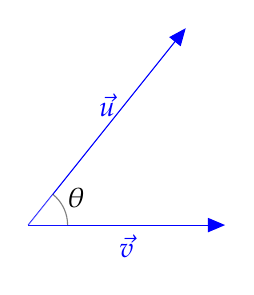
\begin{tikzpicture}
        \coordinate (A) at (0,0);
        \coordinate (X) at (2.5,0);
        \coordinate (Y) at (2,2.5);

        \draw[->,>=triangle 45,color=blue] (A) -- (X)
          node[midway,below]{$\vec{v}$};
        \draw[->,>=triangle 45,color=blue] (A) -- (Y)
          node[midway,above]{$\vec{u}$};
      % \draw[dashed,->,>=triangle 45] (X) -- (Y)
        % node[midway,above right]{$\vec{u} - \vec{v}$};

        % Mark the angle XAY
        \begin{scope}
          \path[clip] (A) -- (X) -- (Y);
          \fill[white, opacity=0.5, draw=black] (A) circle (5mm);
          \node at ($(A)+(30:7mm)$) {$\theta$};
        \end{scope}
    \end{tikzpicture}
\end{document}